\chapter{Soluția propusă}
\label{cap:cap3}

Soluția propusă este o aplicație Python modulară pentru tranzacționare algoritmică pe piața Forex. Proiectul a fost conceput astfel încât aceeași logică decizională să poată fi utilizată atât în testarea istorică, cât și în rularea live controlată. Cele două moduri principale de funcționare sunt \textit{backtest}, pentru simularea strategiilor pe date istorice, și \textit{live}, pentru paper trading prin Interactive Brokers.

În ambele cazuri, deciziile sunt generate printr-un flux comun: datele sunt pregătite, este identificat regimul de piață, strategiile produc semnale, allocatorul agregă aceste semnale, iar componenta de risc stabilește dacă poziția propusă poate fi deschisă. Această organizare reduce duplicarea logicii și permite compararea mai coerentă între rezultatele obținute în backtesting și comportamentul observat în rularea live.

\section{Cerințe funcționale și nefuncționale}
\label{cap:cap3:cerinte}

Aplicația trebuie să permită rularea unui backtest pentru o pereche valutară, un interval de timp, o dată de început și o dată de final. Utilizatorul poate configura capitalul inițial, riscul pe tranzacție, slippage-ul, directorul de cache și directorul de ieșire. Din punct de vedere funcțional, sistemul trebuie să poată descărca sau reutiliza date istorice, să genereze tranzacții simulate și să salveze rezultatele într-o formă care poate fi verificată ulterior.

Pentru modul live, aplicația trebuie să se conecteze la TWS sau IB Gateway în regim paper trading, să monitorizeze perechile selectate și să trimită ordine de piață doar dacă toate filtrele sunt îndeplinite. O cerință importantă este prevenirea utilizării accidentale a unui cont real; de aceea configurația implicită acceptă doar porturile paper 7497 și 4002.

Cerințele nefuncționale urmăresc reproductibilitatea, modularitatea și trasabilitatea. Backtest-ul trebuie să poată fi reluat cu aceiași parametri, iar rezultatele trebuie să includă fișiere separate pentru tranzacții, curba capitalului, metrici de risc, metrici de strategie și sumar text. Aceste cerințe au fost formulate pentru ca aplicația să poată fi analizată nu doar ca prototip funcțional, ci și ca sistem tehnic documentabil.

\subsection{Cerințe ale utilizatorului}
\label{cap:cap3:cerinte_utilizator}

Utilizatorul țintă al aplicației este o persoană care dorește să testeze strategii Forex în mod reproductibil, fără a depinde de o interfață grafică complexă și fără a trimite ordine reale înainte de validare. Din această perspectivă, cerințele utilizatorului sunt:

\begin{itemize}
    \item rularea rapidă a unui backtest prin linia de comandă, cu parametri expliciți;
    \item selectarea perechii valutare, a timeframe-ului, a perioadei istorice și a capitalului inițial;
    \item reutilizarea datelor istorice locale pentru a evita descărcări repetate;
    \item obținerea unui sumar ușor de citit după fiecare rulare;
    \item inspectarea tranzacțiilor individuale, a motivelor de intrare și a motivelor de ieșire;
    \item testarea modului live exclusiv pe cont paper Interactive Brokers;
    \item păstrarea rezultatelor în fișiere standard, care pot fi analizate ulterior în Excel, Python sau alte instrumente.
\end{itemize}

\subsection{Cerințe funcționale detaliate}
\label{cap:cap3:cerinte_functionale}

Tabelul \ref{tabel:cerinte_functionale} detaliază funcționalitățile care trebuie asigurate de aplicație pentru ca fluxul de backtesting și rularea live paper să poată fi utilizate într-un mod coerent. Cerințele au fost formulate pornind de la operațiile principale ale utilizatorului: selectarea datelor, generarea semnalelor, aplicarea regulilor de risc, conectarea la broker și obținerea artefactelor de analiză.

\begin{longtable}{|p{2cm}|p{9.2cm}|p{3cm}|}
    \caption{Cerințe funcționale ale sistemului}
    \label{tabel:cerinte_functionale}\\
        \hline
        \textbf{Cod} & \textbf{Descriere} & \textbf{Prioritate} \\
        \hline
        CF1 & Sistemul permite rularea unui backtest pentru o pereche Forex, un timeframe și un interval temporal definite de utilizator, astfel încât scenariile experimentale să poată fi reluate cu aceiași parametri. & Ridicată \\
        \hline
        CF2 & Sistemul încarcă date istorice din cache local sau le descarcă automat atunci când lipsesc, reducând dependența de descărcări repetate și menținând continuitatea procesului de testare. & Ridicată \\
        \hline
        CF3 & Sistemul calculează indicatorii tehnici necesari strategiilor și detectorului de regim, pentru ca deciziile să fie generate pe baza acelorași transformări ale seriilor OHLCV. & Ridicată \\
        \hline
        CF4 & Sistemul combină semnalele strategiilor într-o decizie finală explicabilă, printr-un mecanism de alocare care păstrează contribuția fiecărei strategii. & Ridicată \\
        \hline
        CF5 & Sistemul verifică fiecare intrare prin reguli de risc înainte de deschiderea poziției, incluzând validarea semnalului, dimensiunea poziției și limitele de expunere. & Ridicată \\
        \hline
        CF6 & Sistemul salvează rapoarte CSV, sumar text și dashboard-uri după fiecare rulare, pentru ca rezultatele să poată fi inspectate, arhivate și comparate ulterior. & Medie \\
        \hline
        CF7 & Sistemul permite conectarea la Interactive Brokers doar în regim paper trading, prevenind utilizarea accidentală a unui cont real în etapa de testare. & Ridicată \\
        \hline
        CF8 & Sistemul expune metrici live pentru monitorizare prin Prometheus și vizualizare în Grafana, astfel încât prețurile, semnalele și starea pozițiilor să poată fi urmărite în timp real. & Medie \\
        \hline
\end{longtable}

\subsection{Cerințe nefuncționale detaliate}
\label{cap:cap3:cerinte_nefunctionale}

Cerințele nefuncționale stabilesc proprietățile de calitate urmărite în implementare. În cazul unei aplicații de tranzacționare algoritmică, aceste cerințe sunt importante deoarece sistemul trebuie să fie reproductibil, ușor de auditat și suficient de sigur pentru a evita execuții nedorite în medii reale.

\begin{longtable}{|p{2cm}|p{9.2cm}|p{3cm}|}
    \caption{Cerințe nefuncționale ale sistemului}
    \label{tabel:cerinte_nefunctionale}\\
        \hline
        \textbf{Cod} & \textbf{Descriere} & \textbf{Categorie} \\
        \hline
        CNF1 & Rulările de backtesting trebuie să fie reproductibile pentru aceleași date și aceiași parametri, pentru ca rezultatele să poată fi verificate independent. & Reproductibilitate \\
        \hline
        CNF2 & Modulele trebuie să poată fi extinse fără modificarea întregului sistem, astfel încât o strategie nouă sau o regulă de risc nouă să poată fi integrată controlat. & Mentenabilitate \\
        \hline
        CNF3 & Deciziile trebuie să poată fi auditate prin fișierele generate, incluzând tranzacțiile, motivele de intrare sau ieșire și evoluția capitalului. & Trasabilitate \\
        \hline
        CNF4 & Aplicația trebuie să prevină conectarea accidentală la porturi non-paper Interactive Brokers, pentru a limita riscul operațional în etapa de testare. & Siguranță operațională \\
        \hline
        CNF5 & Erorile de conexiune live trebuie tratate prin mesaje clare și reconectare controlată, astfel încât utilizatorul să poată identifica rapid cauza întreruperii. & Fiabilitate \\
        \hline
        CNF6 & Serviciile auxiliare de monitorizare trebuie să poată rula pe porturi non-default pentru evitarea conflictelor locale cu alte instanțe Prometheus sau Grafana. & Operabilitate \\
        \hline
\end{longtable}

\section{Alegerea tehnologiilor}
\label{cap:cap3:tehnologii}

Implementarea a fost realizată în Python deoarece limbajul are un ecosistem matur pentru analiză de date, integrare cu API-uri externe și prototipare rapidă. Bibliotecile \texttt{pandas} \cite{misc:web:pandas_docs} și \texttt{NumPy} \cite{misc:web:numpy_docs} sunt utilizate pentru prelucrarea seriilor de timp, calculul indicatorilor și agregarea rezultatelor. \texttt{PyYAML} permite separarea parametrilor de configurare de codul sursă, iar \texttt{dukascopy-python} asigură accesul la date istorice Forex \cite{misc:web:dukascopy_python}. Pentru modul live, \texttt{ib\_insync} oferă o interfață Python peste API-ul Interactive Brokers \cite{misc:web:ib_insync,misc:web:ibkr_api}. Monitorizarea live utilizează \texttt{prometheus-client}, Prometheus, Grafana și Docker Compose pentru colectarea, stocarea și vizualizarea metricilor operaționale \cite{misc:web:prometheus_docs,misc:web:grafana_docs,misc:web:docker_compose_docs}.

Alegerea unei aplicații de tip CLI, în locul unei interfețe grafice, este justificată de caracterul experimental al proiectului. Parametrii pot fi salvați în comenzi reproductibile, rulările pot fi automatizate, iar rezultatele sunt persistate în fișiere.

\begin{table}[htbp]
    \centering
    \caption{Tehnologii utilizate și rolul acestora}
    \label{tabel:tehnologii}
    \begin{tabular}{|p{3.5cm}|p{5cm}|p{5.2cm}|}
        \hline
        \textbf{Tehnologie} & \textbf{Rol în proiect} & \textbf{Justificare} \\
        \hline
        Python & Limbaj principal de implementare & Ecosistem puternic pentru date financiare și prototipare. \\
        \hline
        pandas / NumPy & Prelucrare date, indicatori, tabele de rezultate & Performanță suficientă pentru backtesting pe date OHLCV și API familiar. \\
        \hline
        Dukascopy & Sursă de date istorice Forex & Date accesibile și potrivite pentru cache local. \\
        \hline
        Interactive Brokers & Broker pentru paper trading & Permite testare operațională fără expunere financiară reală. \\
        \hline
        Prometheus / Grafana & Observabilitate live & Colectează metrici expuse de bot și le afișează în dashboard-uri per paritate. \\
        \hline
        Docker Compose & Orchestrare locală monitorizare & Pornește Prometheus și Grafana izolat de mediul Python al botului. \\
        \hline
        CSV / HTML / SVG & Formate de raportare & Ușor de inspectat, arhivat și analizat ulterior. \\
        \hline
    \end{tabular}
\end{table}

\section{Arhitectura sistemului}
\label{cap:cap3:arhitectura}

Figura \ref{fig:arhitectura_sistem} prezintă arhitectura generală a sistemului. Aplicația este organizată în module cu responsabilități clare: interfață CLI, configurare, date, strategii, nucleu decizional, backtesting, live trading și raportare.

Arhitectura a fost gândită astfel încât fluxurile de backtesting și live paper să folosească aceleași componente de decizie, acolo unde acest lucru este posibil. Această alegere reduce diferențele dintre simulare și rularea operațională: strategiile, detectorul de regim, allocatorul și componenta de risc sunt reutilizate, iar diferența principală rămâne sursa datelor și modul de execuție a ordinelor. În acest fel, o modificare asupra logicii de tranzacționare poate fi testată întâi istoric și apoi verificată în mod paper fără rescrierea fluxului decizional.

Separarea modulelor are și un rol de mentenanță. De exemplu, înlocuirea furnizorului de date istorice nu ar trebui să afecteze strategiile, iar adăugarea unei strategii noi nu ar trebui să modifice modulul de raportare. Această structură este importantă într-un sistem experimental, deoarece permite dezvoltarea incrementală și izolarea problemelor atunci când rezultatele unei rulări nu sunt cele așteptate.

\begin{figure}[htbp]
    \centering
    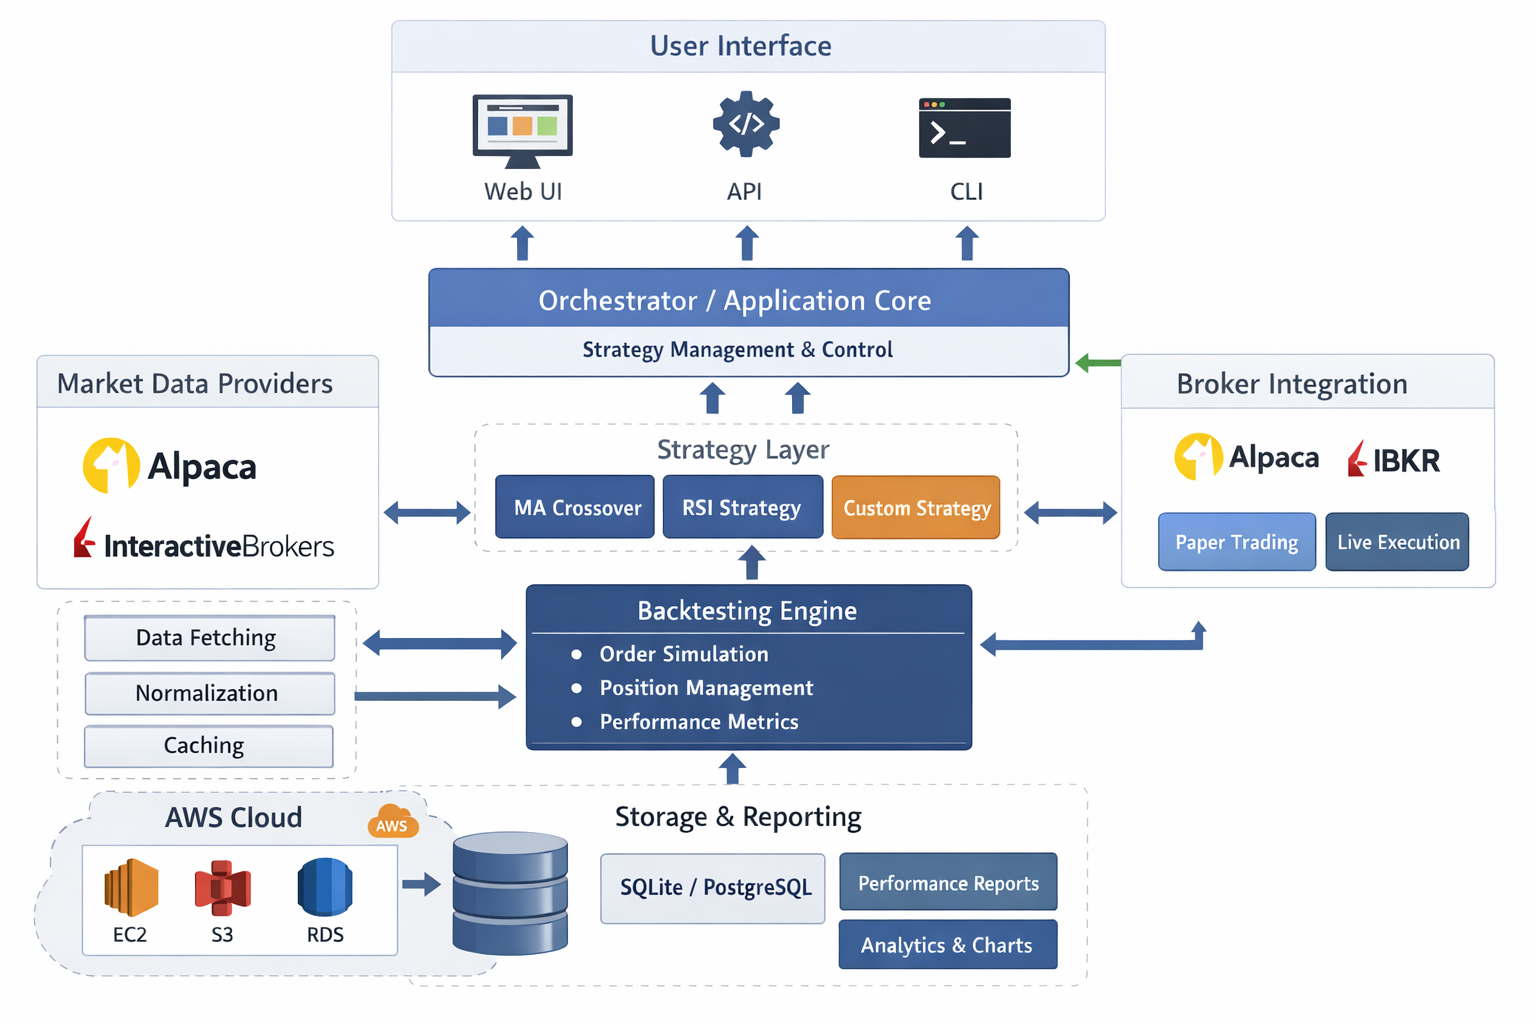
\includegraphics[width=0.95\textwidth]{coperti/arhitectura_sistem.png}
    \caption{Arhitectura sistemului de tranzacționare algoritmică}
    \label{fig:arhitectura_sistem}
\end{figure}

În directorul \texttt{forex\_quant\_bot}, componentele principale sunt:
\begin{itemize}
    \item \texttt{backtest}: motorul de simulare și calculul rapoartelor;
    \item \texttt{core}: detectorul de regim, allocatorul, componenta de risc și tracker-ul de performanță;
    \item \texttt{data}: descărcarea, cache-ul și replay-ul cronologic al datelor;
    \item \texttt{live}: integrarea cu Interactive Brokers și orchestrarea modului live;
    \item \texttt{logs}: persistarea artefactelor CSV, HTML, SVG și text;
    \item \texttt{strategies}: strategiile de trend, mean reversion și breakout;
    \item \texttt{settings.py}: clasele de configurare și suprascrierile per pereche valutară;
    \item \texttt{cli.py}: parsarea parametrilor din linia de comandă și selectarea modului de rulare.
\end{itemize}

\subsection{Responsabilitățile modulelor}
\label{cap:cap3:responsabilitati}

Datele OHLCV sunt obținute și normalizate în modulul \texttt{data}. Clasa \texttt{DataCache} verifică fișierele locale, validează acoperirea temporală și declanșează descărcarea datelor atunci când este necesar. Această separare este importantă deoarece motorul de backtesting primește doar un set de date ordonat cronologic, fără să depindă de detaliile furnizorului extern.

Strategiile propriu-zise sunt grupate în modulul \texttt{strategies}. Fiecare strategie pregătește indicatorii necesari și evaluează istoricul disponibil la momentul curent. Rezultatul este un obiect \texttt{StrategyDecision}, care include semnalul, încrederea și metadatele explicative. Această structură face posibilă adăugarea unei noi strategii fără modificarea motorului de simulare.

Modulul \texttt{core} grupează componentele comune ale deciziei. Detectorul de regim adaugă contextul de piață, allocatorul stabilește ponderea semnalelor, tracker-ul calculează performanța recentă, iar componenta de risc verifică dacă semnalul poate fi transformat în poziție.

Modulul \texttt{backtest} orchestrează simularea. El parcurge barele istorice în ordine cronologică, verifică pozițiile deschise, evaluează strategiile, aplică riscul și salvează tranzacțiile. Modulul \texttt{live} reutilizează aceeași logică decizională, dar înlocuiește sursa de date cu fluxuri Interactive Brokers și transformă intrările/ieșirile în ordine paper.

\subsection{Modelul datelor interne}
\label{cap:cap3:model_date}

Datele și deciziile importante sunt reprezentate prin clase de tip \texttt{dataclass}. Această alegere oferă o structură clară, cu atribute explicite, fără complexitatea unei ierarhii de clase inutile. Printre modelele principale se află:

\begin{itemize}
    \item \texttt{StrategyDecision}: semnalul unei strategii, încrederea și metadatele aferente;
    \item \texttt{CompositeDecision}: semnalul final rezultat din allocator;
    \item \texttt{RiskDecision}: aprobarea sau respingerea unei intrări și motivul deciziei;
    \item \texttt{Position}: starea unei poziții deschise;
    \item \texttt{TradeRecord}: tranzacția închisă, folosită pentru metrici;
    \item \texttt{TradeEventRecord}: evenimentele individuale de intrare și ieșire.
\end{itemize}

Prin aceste structuri, sistemul păstrează o separare clară între semnal, decizie de risc, poziție și rezultat final. Această separare ajută la auditarea rulărilor: dacă o tranzacție este respinsă, motivul se regăsește în decizia de risc; dacă o tranzacție este deschisă, motivul semnalului se păstrează în înregistrarea poziției și apoi în fișierul \texttt{trades.csv}.

\begin{figure}[htbp]
    \centering
    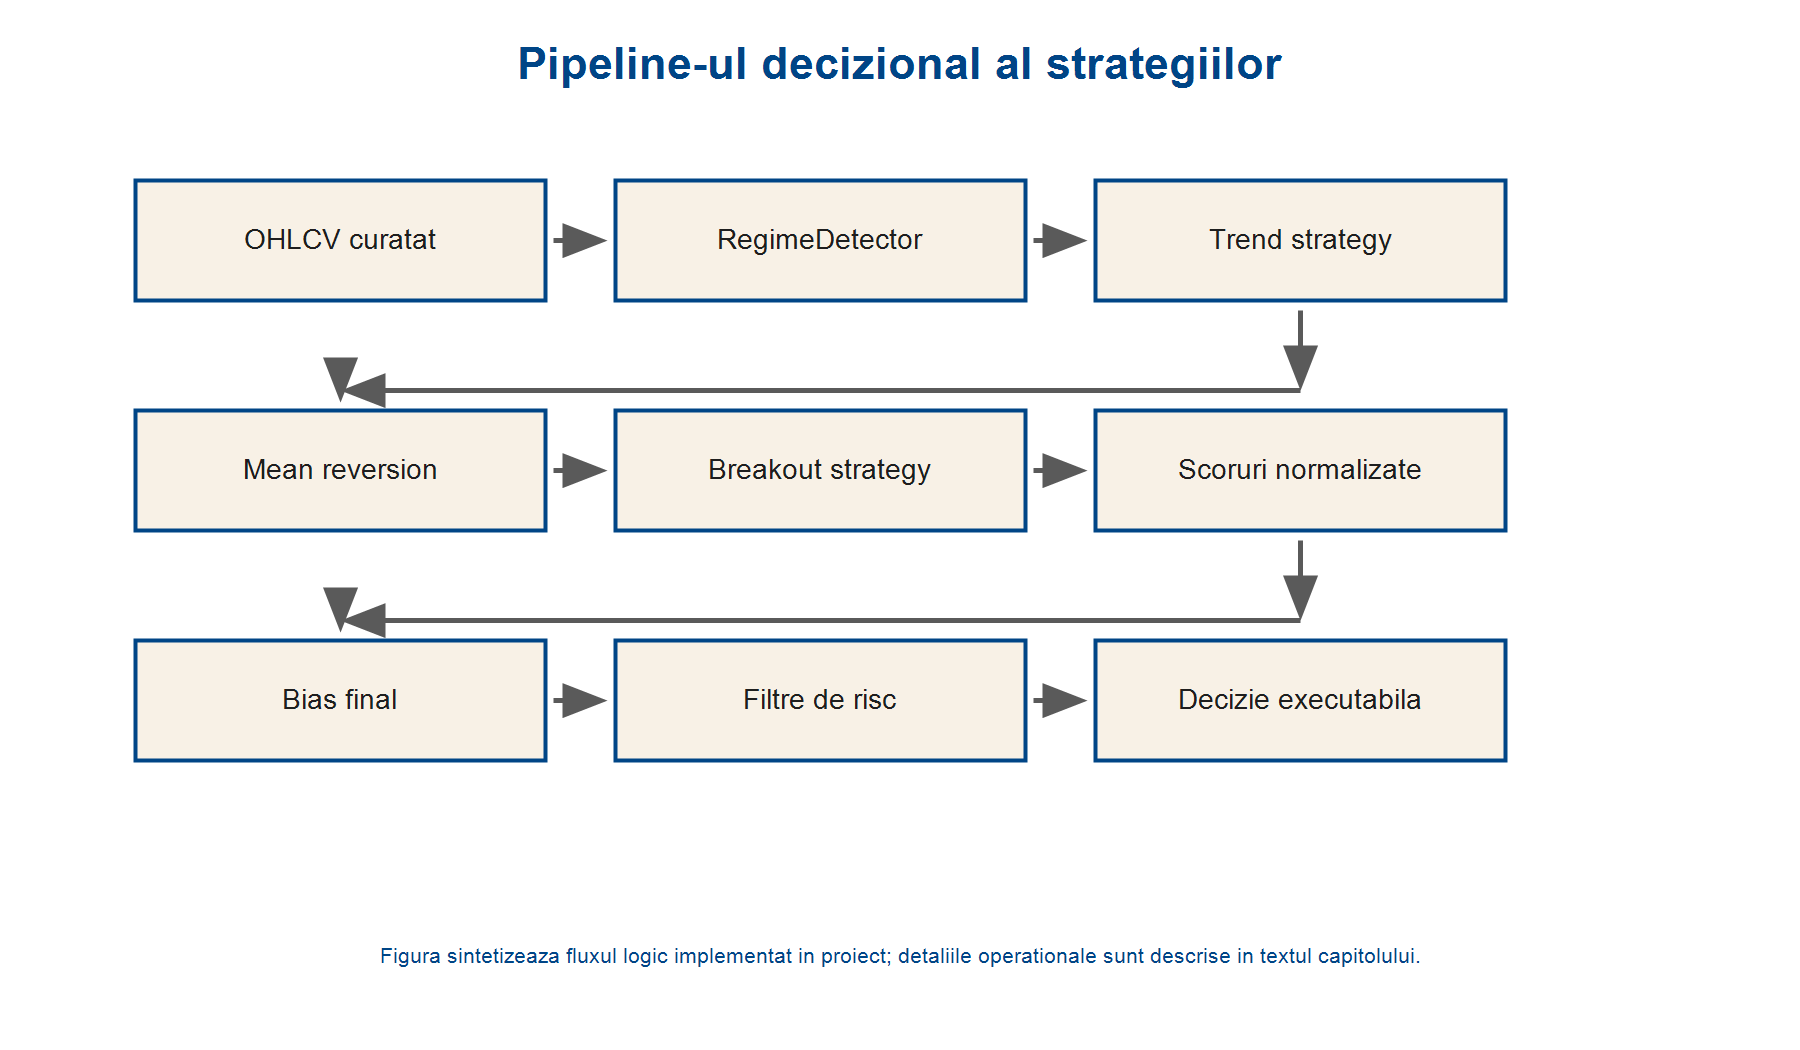
\includegraphics[width=0.95\textwidth]{continut/capitol3/figuri/pipeline_strategii.png}
    \caption{Pipeline-ul decizional al strategiilor}
    \label{fig:pipeline_strategii}
\end{figure}

\section{Trasabilitatea cerințelor}
\label{cap:cap3:trasabilitate}

Tabelul \ref{tabel:trasabilitate_cerinte} leagă cerințele principale de modulele responsabile și de artefactele prin care implementarea poate fi verificată.

\begin{table}[H]
    \centering
    \caption{Trasabilitatea cerințelor către modulele implementate}
    \label{tabel:trasabilitate_cerinte}
    \begin{tabular}{|p{4.2cm}|p{5.2cm}|p{4.6cm}|}
        \hline
        \textbf{Cerință} & \textbf{Componentă responsabilă} & \textbf{Dovadă în proiect} \\
        \hline
        Backtesting reproductibil & \texttt{BacktestEngine}, \texttt{BarReplay}, \texttt{DataCache} & Rulări deterministe pe CSV și directoare timestamped în \texttt{output}. \\
        \hline
        Strategii extensibile & \texttt{BaseStrategy} și modulele din \texttt{strategies} & Fiecare strategie implementează \texttt{prepare\_data} și \texttt{evaluate}. \\
        \hline
        Decizie explicabilă & \texttt{StrategyAllocator}, \texttt{StrategyDecision} & Scoruri pe strategie, metadate și motivul semnalului în CSV-uri. \\
        \hline
        Controlul riscului & \texttt{RiskOverlay}, \texttt{RiskConfig} & Stop-uri ATR, sizing, expunere maximă și circuit breaker. \\
        \hline
        Integrare broker & \texttt{IBPaperBroker}, \texttt{LiveRunner} & Validare porturi paper 7497/4002 și lock-uri pe pereche. \\
        \hline
        Raportare completă & \texttt{CSVLogger}, \texttt{SummaryPrinter}, \texttt{performance\_dashboard} & Fișiere CSV, sumar text, HTML și SVG după rulare. \\
        \hline
    \end{tabular}
\end{table}

\section{Fluxul de backtesting}
\label{cap:cap3:backtest}

În modul backtest, utilizatorul pornește aplicația printr-o comandă de forma:

\begin{code}
\begin{minted}{bash}
python main.py --mode backtest --pair EURUSD --start 2018-01-01 \
  --end 2024-12-31 --timeframe D
\end{minted}
\caption{Exemplu de comandă pentru rularea unui backtest}
\label{code:backtest_command}
\end{code}

Motorul verifică existența datelor în directorul \texttt{data\_cache}. Dacă acoperirea temporală este suficientă, fișierul CSV local este reutilizat. În caz contrar, datele sunt descărcate prin Dukascopy, dacă descărcarea automată este activă. Datele sunt apoi adnotate cu indicatori de regim și cu indicatorii specifici fiecărei strategii.

Procesarea se face bară cu bară. Pentru fiecare moment, motorul actualizează poziția curentă, verifică stop-loss-ul și take-profit-ul, evaluează strategiile și transmite semnalul compus către componenta de risc. Dacă riscul este aprobat, este creată o poziție nouă. Dacă există deja o poziție, aceasta poate fi închisă prin stop, take-profit, trailing stop, break-even sau semnal opus.

Fragmentul următor sintetizează fluxul de decizie folosit în backtesting. El evidențiază faptul că strategiile sunt evaluate pe istoricul disponibil la momentul curent, iar decizia compusă este transmisă separat către componenta de risc.

\begin{code}
\begin{minted}[basicstyle=\footnotesize\ttfamily\bfseries\color{codeIdentifier}]{python}
for event in BarReplay(market_data, warmup_bars=warmup_bars):
    bar = event.bar
    close_price = float(bar["close"])

    decisions = {
        strategy.name: strategy.evaluate(event.history)
        for strategy in strategies
    }
    composite = allocator.allocate(
        decisions,
        current_regime=str(bar["regime"]),
        performance_tracker=tracker,
    )

    risk_decision = risk_overlay.evaluate_entry(
        pair=pair,
        open_positions=[],
        bias=composite.bias,
        equity=equity,
        current_open_risk_ratio=open_risk_ratio,
        close_price=close_price,
        atr_value=float(bar["atr"]),
        quote_to_usd_rate=quote_to_usd,
    )
\end{minted}
\caption{Sinteză a fluxului de decizie din backtesting}
\label{code:flux_decizie_backtest}
\end{code}

\begin{figure}[htbp]
    \centering
    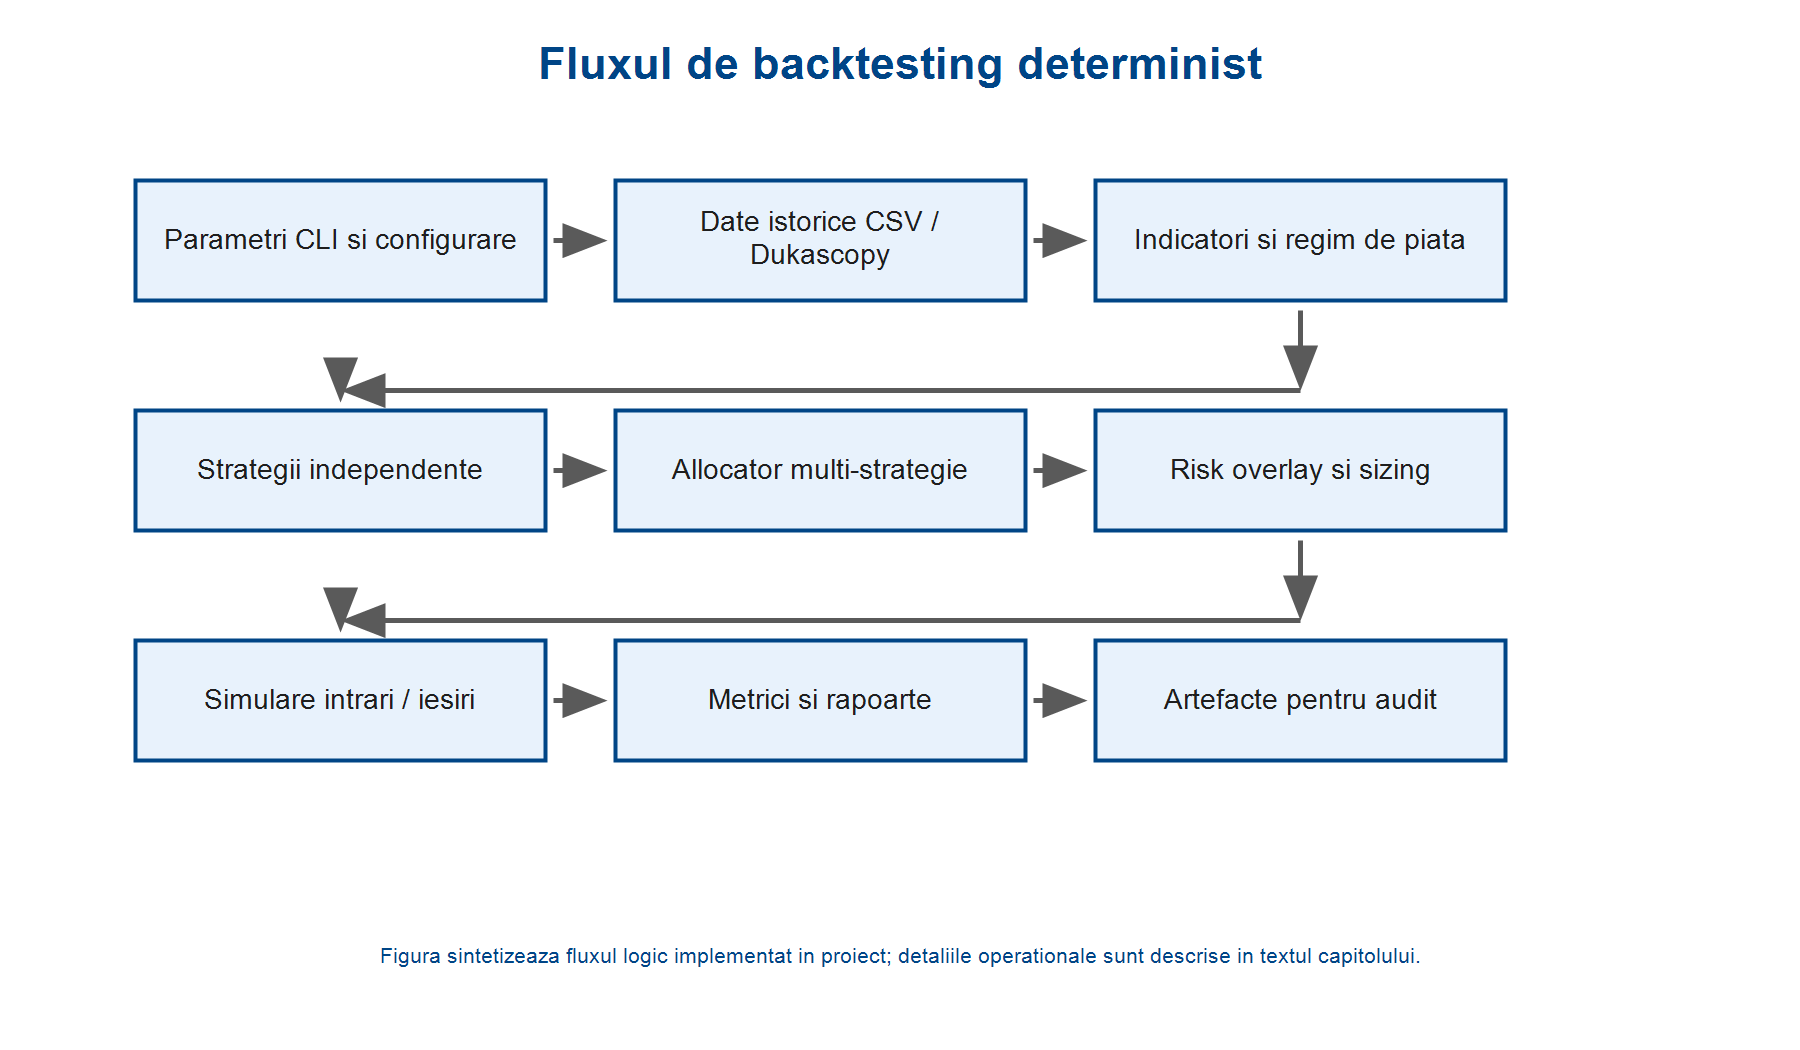
\includegraphics[width=0.95\textwidth]{continut/capitol3/figuri/flux_backtesting.png}
    \caption{Fluxul de backtesting determinist}
    \label{fig:flux_backtesting}
\end{figure}

\section{Strategiile implementate}
\label{cap:cap3:strategii}

Sistemul include trei strategii complementare.

\textit{Strategia de trend} folosește EMA rapidă și lentă, ADX, MACD și confirmare multi-timeframe. Ea produce semnal long în regim \textit{trend\_up}, când EMA rapidă este peste EMA lentă, ADX depășește pragul configurat, iar MACD confirmă direcția. Pentru semnal short sunt verificate condiții simetrice în regim \textit{trend\_down}.

\textit{Strategia de revenire la medie} folosește Bollinger Bands, RSI și filtre de calitate a lumânării. Ea este activă doar în regim \textit{range}, cu ADX scăzut și volatilitate controlată. Semnalele apar când prețul se află la extremele canalului statistic, iar RSI indică supravânzare sau supracumpărare.

\textit{Strategia de breakout} folosește canale Donchian și ATR. Ea caută închideri peste maximul canalului sau sub minimul canalului anterior, dar acceptă tranzacții doar când volatilitatea este suficient de ridicată. Această strategie este potrivită pentru trenduri și pentru episoade de creștere bruscă a volatilității.

Complementaritatea strategiilor este importantă deoarece piața Forex nu rămâne permanent într-un singur comportament. O strategie de trend poate avea rezultate slabe într-o piață laterală, în timp ce o strategie de revenire la medie poate produce semnale greșite în timpul unui breakout puternic. Prin urmare, sistemul nu alege manual o singură strategie pentru toate perioadele, ci permite allocatorului să acorde ponderi diferite în funcție de performanță și context.

\begin{table}[H]
    \centering
    \small
    \setlength{\tabcolsep}{4pt}
    \renewcommand{\arraystretch}{1.15}
    \caption{Rezumatul strategiilor implementate}
    \label{tabel:strategii_rezumat}
    \begin{tabular}{|p{2.8cm}|p{4.1cm}|p{3.2cm}|p{3.7cm}|}
        \hline
        \textbf{Strategie} & \textbf{Indicatori utilizați} & \textbf{Regim țintă} & \textbf{Rol în sistem} \\
        \hline
        Trend & EMA, ADX, MACD, confirmare multi-timeframe & \texttt{trend\_up}, \texttt{trend\_down} & Urmărește mișcări direcționale persistente. \\
        \hline
        Mean reversion & Bollinger Bands, RSI, ADX, filtre de lumânare & \texttt{range} & Caută revenirea prețului de la extreme statistice. \\
        \hline
        Breakout & Donchian Channels, ATR, z-score volatilitate & trend sau \texttt{volatility\_spike} & Caută străpungeri ale canalelor de preț. \\
        \hline
    \end{tabular}
    \renewcommand{\arraystretch}{1.0}
\end{table}

\section{Allocatorul de strategii}
\label{cap:cap3:allocator}
\label{sec:allocator}

Fiecare strategie returnează un semnal, o încredere și metadate explicative. Allocatorul combină semnalele printr-un scor compus. Pentru fiecare strategie sunt evaluate patru componente:
\begin{itemize}
    \item performanța recentă, calculată din win rate, profit factor, profit mediu și drawdown;
    \item încrederea declarată de strategie pentru semnalul curent;
    \item potrivirea cu regimul de piață;
    \item diversificarea față de istoricul semnalelor celorlalte strategii.
\end{itemize}

Scorul compus folosește ponderile 0,4 pentru performanță, 0,3 pentru încredere, 0,2 pentru potrivirea cu regimul și 0,1 pentru diversificare. Semnalul final este suma semnalelor individuale ponderate cu scorurile normalizate. Dacă valoarea finală depășește pragul configurat, bias-ul devine long; dacă scade sub pragul negativ, bias-ul devine short; în caz contrar sistemul rămâne flat.

Ponderile allocatorului sunt definite ca parametri de configurare. Valorile implicite reflectă o ierarhie de proiectare: performanța recentă are ponderea cea mai mare, deoarece sistemul trebuie să favorizeze strategiile care au demonstrat rezultate mai bune în contextul curent; încrederea semnalului are a doua pondere, deoarece descrie forța condițiilor tehnice identificate de strategie; potrivirea cu regimul de piață ajustează decizia în funcție de context, iar diversificarea are rol de corecție pentru a evita concentrarea excesivă pe strategii care produc semnale similare.

Această alegere nu trebuie interpretată ca optimizare empirică definitivă. Ea reprezintă o configurație inițială, explicabilă și ușor de modificat. Sistemul permite testarea altor combinații, precum 0,3/0,3/0,2/0,2, fără modificarea codului sursă. O variantă mai avansată ar fi folosirea unor ponderi adaptive, actualizate în funcție de volatilitate, regim de piață sau performanță out-of-sample, însă această direcție a fost păstrată pentru dezvoltări ulterioare.

Rolul allocatorului este de a evita dependența excesivă de o singură strategie. În loc ca sistemul să aleagă permanent aceeași logică de tranzacționare, fiecare strategie contribuie în funcție de context și de performanța sa recentă. Astfel, o strategie care a avut rezultate slabe într-un anumit regim primește o influență mai mică, iar o strategie mai potrivită condițiilor curente poate avea o pondere mai mare.

Această abordare nu garantează eliminarea semnalelor greșite, dar oferă o formă de adaptare controlată. Decizia finală rămâne explicabilă, deoarece scorurile pe strategie și componentele folosite la calcul pot fi salvate și analizate ulterior. Pentru o lucrare tehnică, această transparență este importantă: nu este suficient ca sistemul să producă un semnal, ci trebuie să se poată explica de ce acel semnal a fost preferat.

\section{Managementul riscului}
\label{cap:cap3:risk_overlay}

Componenta \texttt{RiskOverlay} decide dacă un semnal poate fi executat. Prima verificare este starea circuit breaker-ului. Dacă drawdown-ul curent a depășit pragul configurat, tranzacționarea este dezactivată temporar. Apoi sunt validate prețul, ATR-ul, cursul de conversie către USD, nivelul de volatilitate și expunerea pe monede.

Dimensiunea poziției este calculată pornind de la riscul dorit:

\begin{equation}
    \label{eq:position_size}
    size = \frac{equity \cdot risk\_per\_trade}{ATR \cdot atr\_multiplier \cdot quote\_to\_usd}
\end{equation}

Formula \eqref{eq:position_size} este limitată suplimentar de expunerea maximă și de levierul noțional maxim. Stop-loss-ul este plasat la o distanță de ATR față de prețul de intrare, iar take-profit-ul este stabilit la o distanță mai mare, pentru a permite raporturi risc-recompensă favorabile. Pe parcursul tranzacției, sistemul poate muta stop-ul la break-even și poate activa trailing stop-ul.

Implementarea practică păstrează aceeași logică: se calculează suma maximă riscată, riscul pe unitate și dimensiunea permisă atât de risc, cât și de levierul noțional. Dimensiunea finală este minimul dintre cele două limite.

\begin{code}
\begin{minted}[basicstyle=\footnotesize\ttfamily\bfseries\color{codeIdentifier}]{python}
target_risk_amount = equity * self.config.risk_per_trade
stop_distance = atr_value * self.config.atr_stop_multiplier
usd_risk_per_unit = stop_distance * quote_to_usd_rate

size_by_risk = int(max(target_risk_amount / usd_risk_per_unit, 1))
max_notional_usd = equity * self.config.max_notional_leverage
size_by_notional = int(max(max_notional_usd / usd_notional_per_unit, 0))

size_units = min(size_by_risk, size_by_notional)
\end{minted}
\caption{Dimensionarea poziției în funcție de risc și volatilitate}
\label{code:position_size_risc}
\end{code}

Regulile de risc nu sunt tratate ca o extensie a strategiilor, ci ca o componentă independentă. Această decizie de proiectare reduce riscul ca o strategie să își suprascrie propriile protecții și permite verificarea uniformă a tuturor semnalelor. De exemplu, indiferent dacă semnalul provine din trend sau din breakout, intrarea poate fi respinsă pentru volatilitate insuficientă, lichiditate anormală, expunere prea mare sau circuit breaker activ.

\begin{table}[H]
    \centering
    \footnotesize
    \setlength{\tabcolsep}{4pt}
    \renewcommand{\arraystretch}{1.5}
    \caption{Motive posibile de respingere a unei intrări}
    \label{tabel:motive_respingere_risc}
    \begin{tabular}{|p{4.4cm}|p{7.6cm}|}
        \hline
        \textbf{Motiv} & \textbf{Semnificație} \\
        \hline
        \texttt{flat\_signal} & Allocatorul nu a produs un bias long sau short suficient de puternic. \\
        \hline
        \texttt{invalid\_atr\_or\_price} & Prețul, ATR-ul sau cursul de conversie nu permit calculul riscului. \\
        \hline
        \texttt{quiet\_market\_atr} & Volatilitatea curentă este prea mică față de media recentă. \\
        \hline
        \texttt{liquidity\_range\_spike} & Bara curentă are o amplitudine anormală față de media ultimelor bare. \\
        \hline
        \texttt{max\_exposure} & Deschiderea poziției ar depăși expunerea totală maximă permisă. \\
        \hline
        \texttt{circuit\_breaker} & Drawdown-ul a depășit pragul configurat, iar tranzacționarea este oprită temporar. \\
        \hline
    \end{tabular}
    \renewcommand{\arraystretch}{1.0}
\end{table}

\section{Modul live paper trading}
\label{cap:cap3:live}

Modul live folosește Interactive Brokers prin biblioteca \textit{ib\_insync}. La pornire, sistemul se conectează la broker, încarcă date istorice pentru încălzirea indicatorilor și pornește fluxurile de bare și prețuri. Pentru fiecare bară completă, fluxul decizional este similar cu cel din backtest. Diferența principală este că intrările și ieșirile sunt trimise brokerului ca ordine de piață, iar prețul de execuție este preluat din răspunsul brokerului.

Sistemul include mecanisme operaționale importante: lock-uri locale pentru a preveni rularea mai multor procese pe aceeași pereche și același cont, heartbeat pentru conexiunea Interactive Brokers, detectarea lipsei de actualizări și reconectare automată. Aceste mecanisme nu garantează absența riscului operațional, dar cresc robustețea în mediu paper.

În modul live, aplicația nu urmărește optimizarea vitezei de execuție, ci verificarea controlată a comportamentului operațional. Aceasta înseamnă că accentul este pus pe siguranța conexiunii, pe observarea stării sistemului și pe confirmarea faptului că semnalele generate de logica internă pot fi transformate în ordine paper. Pentru scopul lucrării, acest nivel de validare este potrivit, deoarece demonstrează integrarea cu brokerul fără a introduce riscul financiar al unui cont real.

Încălzirea indicatorilor înainte de procesarea barelor live este necesară deoarece strategiile folosesc medii mobile, ATR, ADX și alte valori calculate pe ferestre istorice. Dacă sistemul ar porni fără istoric suficient, primele semnale ar putea fi instabile sau incomplete. Prin încărcarea datelor istorice la pornire, modul live pornește dintr-o stare mai apropiată de cea a backtesting-ului.

\begin{figure}[htbp]
    \centering
    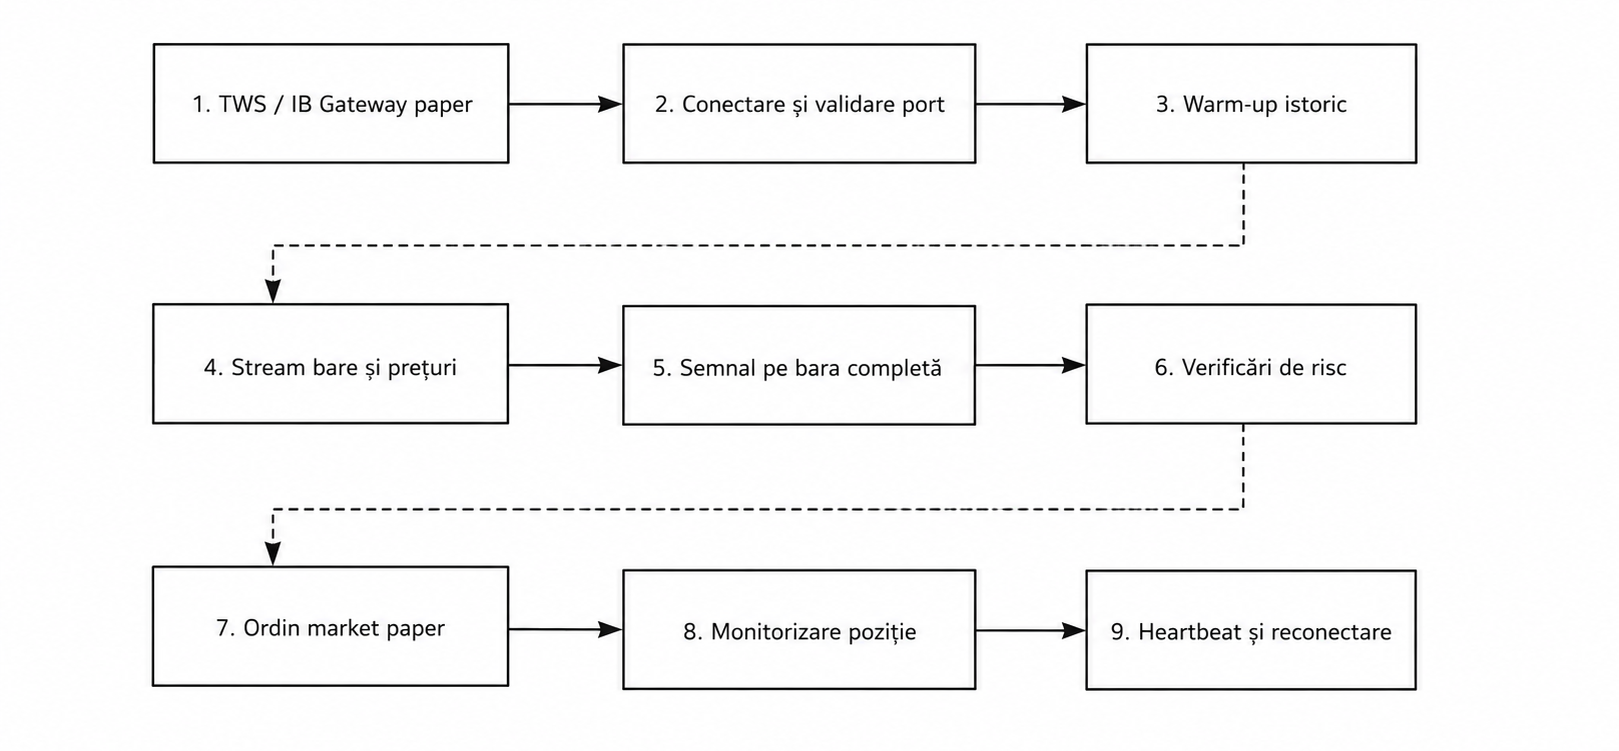
\includegraphics[width=0.95\textwidth]{continut/capitol3/figuri/flux_live_paper.png}
    \caption{Fluxul de rulare live paper prin Interactive Brokers}
    \label{fig:flux_live_paper}
\end{figure}

\section{Observabilitate în timp real}
\label{cap:cap3:observabilitate}
\label{sec:monitorizare}

Pentru modul live, proiectul include un mecanism de observabilitate bazat pe Prometheus și Grafana. Botul pornește local un server HTTP de metrici pe portul \texttt{18000}, iar Prometheus colectează valorile la un interval de 5 secunde prin ținta \texttt{host.docker.internal:18000}. Grafana citește datele din Prometheus și prezintă dashboard-uri separate pentru EURUSD, GBPUSD și USDJPY.

Au fost definite metrici globale și metrici pe pereche valutară. Metricile globale urmăresc capitalul curent, profitul/pierderea realizată și numărul total de poziții deschise. Metricile etichetate cu \texttt{pair} urmăresc prețul live, semnalul allocatorului, poziția deschisă, dimensiunea poziției și P\&L-ul realizat/nerealizat pentru fiecare paritate. Această separare permite analiza independentă a fiecărei perechi, fără amestecarea seriilor într-un singur grafic.

Serviciile de monitorizare rulează prin Docker Compose pe porturi non-default, pentru a evita conflictele cu alte aplicații locale: Grafana este expusă în browser la \texttt{localhost:33000}, Prometheus la \texttt{localhost:39090}, iar exporter-ul botului la \texttt{localhost:18000/metrics}. În interiorul rețelei Docker, Grafana accesează Prometheus prin adresa \texttt{http://prometheus:9090}, deoarece acesta este portul intern al containerului, nu portul publicat pe sistemul gazdă.

Observabilitatea este utilă mai ales în modul live, deoarece anumite probleme nu sunt vizibile doar din fișierele generate la final. De exemplu, lipsa actualizării prețului, menținerea unei poziții deschise sau apariția unui semnal neașteptat pot fi urmărite în timp real. Prin separarea metricilor pe pereche valutară, dashboard-urile permit identificarea rapidă a instrumentului care produce o abatere, fără a confunda starea globală a botului cu starea unei singure perechi.

Un alt avantaj al monitorizării este verificarea funcționării infrastructurii auxiliare. Pagina de targets din Prometheus confirmă dacă exporter-ul botului este accesibil, iar panourile Grafana arată dacă valorile colectate sunt actualizate. Astfel, monitorizarea nu este doar o componentă vizuală, ci și un instrument de diagnostic pentru rulările live paper.

\section{Configurare, reproductibilitate și trasarea experimentelor}
\label{cap:cap3:reproductibilitate}

Un aspect important al proiectului este posibilitatea de a relua experimentele în condiții cât mai apropiate de cele inițiale. În tranzacționarea algoritmică, rezultatele izolate au valoare redusă dacă nu pot fi reproduse și verificate ulterior. Din acest motiv, aplicația separă explicit codul sursă de parametrii de configurare, iar rulările sunt lansate prin comenzi care includ perechea valutară, timeframe-ul, intervalul istoric, capitalul inițial și parametrii principali de risc.

Fișierele de configurare din directorul \texttt{config} permit definirea perechilor urmărite și ajustarea parametrilor fără modificarea codului. Această abordare reduce riscul introducerii unor erori accidentale în implementare și face mai clară diferența dintre logica sistemului și scenariile experimentale. În plus, setările specifice unei perechi pot fi izolate, ceea ce permite adaptarea controlată a parametrilor pentru EURUSD, GBPUSD sau USDJPY.

Reproductibilitatea este susținută și prin folosirea cache-ului local de date. Odată descărcate, seriile istorice pot fi reutilizate în rulări ulterioare, evitând diferențele care ar putea apărea din cauza actualizărilor furnizorului de date sau a problemelor de conectivitate. În contextul lucrării, această decizie este importantă deoarece permite verificarea acelorași tranzacții și a acelorași artefacte generate.

Fiecare rulare produce un director separat în \texttt{output}, cu un nume care include modul de rulare, perechea valutară, timeframe-ul, intervalul analizat și timestamp-ul execuției. Această organizare facilitează compararea experimentelor și previne suprascrierea rezultatelor anterioare. În plus, fișierele CSV generate pot fi inspectate independent de aplicație, ceea ce întărește caracterul auditabil al proiectului.

\section{Artefacte generate}
\label{cap:cap3:artefacte}

Fiecare rulare generează un director în \texttt{output}. Artefactele principale sunt:
\begin{itemize}
    \item \texttt{trades.csv}: lista tranzacțiilor închise;
    \item \texttt{transactions.csv}: evenimente de intrare și ieșire;
    \item \texttt{equity\_curve.csv}: evoluția capitalului;
    \item \texttt{strategy\_metrics.csv}: performanța strategiilor;
    \item \texttt{regime\_metrics.csv}: performanța pe regimuri de piață;
    \item \texttt{risk\_overlay\_metrics.csv}: deciziile componentei de risc;
    \item \texttt{summary.txt}: raport text cu metricile principale;
    \item \texttt{dashboard.html} și \texttt{performance\_dashboard.svg}: vizualizări pentru analiză.
\end{itemize}

\section{Algoritmul general}
\label{cap:cap3:algoritm}

\begin{algorithm}[H]
    \caption{Fluxul decizional al sistemului}
    \label{alg:flux_decizional}
    \begin{algorithmic}[1]
        \Procedure{RunBot}{config}
            \State Încarcă datele istorice sau fluxul live
            \State Calculează indicatorii și regimul de piață
            \For{fiecare bară completă}
                \State Actualizează poziția deschisă și capitalul
                \State Verifică stop-loss, take-profit, break-even și trailing stop
                \State Evaluează strategiile active
                \State Agregă semnalele prin allocator
                \State Verifică aprobarea componentei de risc
                \If{riscul este aprobat și nu există poziție deschisă}
                    \State Deschide poziție long sau short
                \EndIf
                \State Înregistrează tranzacții, metrici și curba capitalului
            \EndFor
            \State Generează rapoarte CSV, text și dashboard
        \EndProcedure
    \end{algorithmic}
\end{algorithm}
